\chapter{DNA Models}
\label{chap:dna}


\section{3SPN.2C}
\label{sec:dna_3spn2c}

The series of the 3SPN.x DNA models have been developed by de Pablo's group.
The 3SPN.2C model is the one for modeling sequence-dependent curvature of
double-stranded DNA (dsDNA).  Particularly, the model has been well-tuned to
reproduce both mechanical and geometrical properties, such as persistent length
and major/minor groove widths.

\subsection{Topology}
\label{subsec:dna_3spn2c_top}

In this model, each nucleotide is represented by three CG particles, P
(phosphate), S (sugar), and B (base), as shown in
Figure~\ref{fig:dna_3spn2c_top}.  B has four types: A (adenine), C (cytosine), G
(guanine), and T (thymine).  The CG particles are put at the center-of-mass of
each chemical moiety.

\begin{figure}[ht]
  \centering
  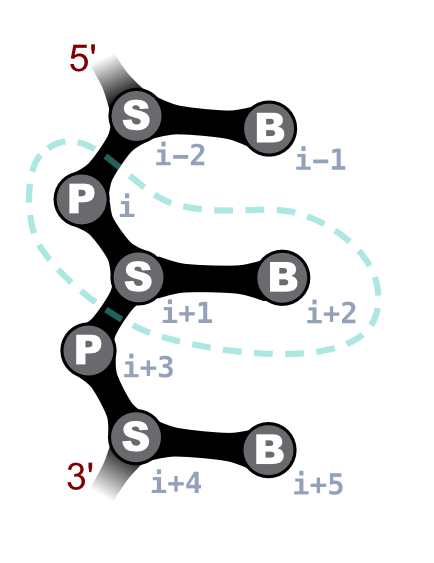
\includegraphics[width=0.3\textwidth]{figures/DNA_3spn2c_top.png}
  \caption{Topology of the 3SPN.2C DNA model: each nucleotide is represented by
    3 sites corresponding to phosphate (P), deoxyribose sugar (S), and
    nitrogenous base (B).  A typical nucleotide ``residue'' is enclosed by the
    dashed line.}
  \label{fig:dna_3spn2c_top}
\end{figure}


\begin{table}[ht]
  \centering
  \begin{tabular}{lc}
    \toprule
    Particle Type    & Mass (amu) \\
    \midrule
    P  &  94.97 \\
    S  &  83.11 \\
    A  &  134.1 \\
    C  &  110.1 \\
    G  &  150.1 \\
    T  &  125.1 \\
    \bottomrule
  \end{tabular}
  \caption{Mass of the 3SPN.2C DNA particles.}
  \label{tab:dna_3spn2c_top_mass}
\end{table}

\subsection{Potentials}
\label{subsec:dna_3spn2c_potential}

The 3SPN.2C potentials can be devided into two parts, as usual, bonded, and
nonbonded:
\begin{displaymath}
  U = U_b + U_{nb}.
\end{displaymath}

The bonded potentials include the following terms:
\begin{itemize}
\item bonds ($U_{bond}$),
\item angles ($U_{ang}$),
\item dihedral angles ($U_{dih}$).
\end{itemize}
\begin{equation}
  \label{eq:dna_3spn2c_local}
  U_b = U_{bond} + U_{ang} + U_{dih}.
\end{equation}

The nonbonded potentials include these terms:
\begin{itemize}
\item base-base interactions:
  \begin{itemize}
  \item base stacking ($U_{bstk}$),
  \item base pairing ($U_{bp}$),
  \item cross base stacking ($U_{cstk}$),
  \end{itemize}
\item excluded volume interactions ($U_{exv}$),
\item electrostatic interactions ($U_{ele}$).
\end{itemize}
\begin{equation}
  \label{eq:dna_3spn2c_nonlocal}
  U_{nb} = U_{bstk} + U_{bp} + U_{cstk} + U_{exv} + U_{ele}.
\end{equation}


\subsubsection{Bond}
\label{sec:dna_3spn2c_potential_bond}

\begin{smallpage}{3SPN.2C bond potential}<white>
  \begin{equation}
    \label{eq:dna_3spn2c_local_bond}
    U_{bond} = \sum_{i}^{bonds} k_b (r_i - r_{i,0})^2 + 100 k_b (r_i - r_{i,0})^4.
  \end{equation}
  \tcblower
  \begin{itemize}
  \item Involved particles:
    \begin{itemize}
    \item P--S
    \item S--B
    \item S--P
    \end{itemize}
  \item $r_{i, 0}$: based on the structure of B-form DNA.
  \item $k_b = 0.6\ \mathrm{kJ/mol/\angstrom^2}$.
  \end{itemize}
\end{smallpage}



\subsubsection{Angle}
\label{sec:dna_3spn2c_potential_angle}

\begin{smallpage}{3SPN.2C bond angle potential}<white>
  \begin{equation}
    \label{eq:dna_3spn2c_local_angle}
    U_{ang} = \sum_{i}^{angles} k_\theta (\theta_i - \theta_{i,0})^2.
  \end{equation}
  \tcblower
  \begin{itemize}
  \item Involved particles:
    \begin{itemize}
    \item P--S--P
    \item S--P--S
    \item P--S--B
    \item B--S--P
    \end{itemize}
  \item $\theta_{i, 0}$: based on the structure of B-form DNA.
  \item $k_\theta$: see the tables below: (unit: $\mathrm{kJ/mol/rad^2}$)
  \end{itemize}
  \begin{center}
    \begin{tabular}{l|cl|cl|cl|cl}
      \toprule
      \emph{PSP} & all & \multicolumn{7}{l}{300}\\
      \midrule
      \multirow{4}{*}{\emph{SPS}} &
                                    AA & 355 & AT & 147 & AC & 464 & AG & 368 \\
                 & TA & 230 & TT & 355 & TC & 442 & TG & 273 \\
                 & CA & 273 & CT & 368 & CC & 165 & CG & 478 \\
                 & GA & 442 & GT & 464 & GC & 228 & GG & 165 \\
      \midrule
      \multirow{4}{*}{\emph{PSB}} &
                                    AA & 460 & TA & 120 & CA & 206 & GA & 383 \\
                 & AT & 370 & TT & 460 & CT & 358 & GT & 442 \\
                 & AC & 442 & TC & 383 & CC & 278 & GC & 336 \\
                 & AG & 358 & TG & 206 & CG & 278 & GG & 278 \\
      \midrule
      \multirow{4}{*}{\emph{BSP}} &
                                    AA & 460 & AT & 370 & AC & 442 & AG & 358 \\
                 & TA & 120 & TT & 460 & TC & 383 & TG & 206 \\
                 & CA & 206 & CT & 358 & CC & 278 & CG & 278 \\
                 & GA & 383 & GT & 442 & GC & 336 & GG & 278 \\
      \bottomrule
    \end{tabular}
  \end{center}
\end{smallpage}

\subsubsection{Dihedral Angle}
\label{sec:dna_3spn2c_potential_dihedral_angle}

The dihedral angle potential in the 3SPN.2C model contains two parts:
\begin{enumerate}
\item A strong Gaussian type potential applied on the backbone dihedrals
  ($U_{dih, Gaussian}$);
\item A weak periodic potential applied on all dihedral angles ($U_{dih, periodic}$).
\end{enumerate}
\begin{equation}
  \label{eq:dna_3spn2c_local_dihedral}
  U_{dih} = U_{dih, Gaussian} + U_{dih, periodic}.
\end{equation}

\begin{smallpage}{3SPN.2C dihedral angle potential (Gaussian)}<white>
  \begin{equation}
    \label{eq:dna_3spn2c_local_dihedral_Gaussian}
    U_{dih, Gaussian} = \sum_{i}^{dihedrals} -k_{ \phi, Gaussian } \exp\big( \frac{-(\phi_i - \phi_{i,0})^2}{2\sigma_{\phi}^2} \big).
  \end{equation}
  \tcblower
  \begin{itemize}
  \item Involved particles:
    \begin{itemize}
    \item P--S--P--S
    \item S--P--S--P
    \end{itemize}
  \item $\phi_{i, 0}$: based on the structure of B-form DNA.
  \item $k_{\phi, Gaussian} = 7.0\ \mathrm{kJ/mol}$.
  \item $\sigma_\phi = 0.3\ \mathrm{rad^2}$.
  \end{itemize}
\end{smallpage}

\begin{smallpage}{3SPN.2C dihedral angle potential (periodic)}<white>
  \begin{equation}
    \label{eq:dna_3spn2c_local_dihedral_periodic}
    U_{dih, periodic} = k_{\phi, periodic} \big[ 1+\cos(\phi_i - \phi_{ i,0 }) \big].
  \end{equation}
  \tcblower
  \begin{itemize}
  \item Involved particles:
    \begin{itemize}
    \item P--S--P--S
    \item S--P--S--P
    \item S--P--S--B
    \item B--S--P--S
    \end{itemize}
  \item $\phi_{i, 0}$: based on the structure of B-form DNA.
  \item $k_{\phi, periodic} = 2.0\ \mathrm{kJ/mol}$.
  \end{itemize}
\end{smallpage}


\subsubsection{Base Stacking Interactions}
\label{sec:dna_3spn2c_potential_bstk}

Before we introduce the nonbonded terms, we would like to first show the
topology of the double stranded DNA and clarify the CG particles involved in the
base-base interaction terms (see Figure~\ref{fig:DNA_3spn2c_nonbonded_all}).

\begin{figure}[ht]
  \centering
  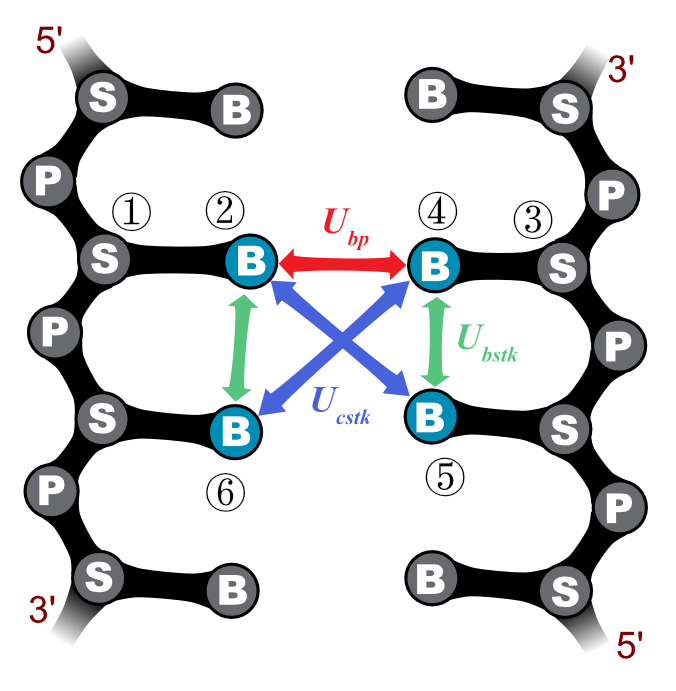
\includegraphics[width=0.45\textwidth]{figures/DNA_3spn2c_nonbonded_all.png}
  \caption{The base-related nonbonded interactions among DNA CG particles.  Here
    we introduce local indices (circled numbers) for easy understanding.  The
    base-stacking interactinos are calculated for the neighboring bases
    ($U_{bstk}$).  The base-pairing interactions are considered for Watson-Crick
    pairs, namely, the A-T and G-C pairs ($U_{bp}$).  Whereas the cross-stacking
    terms are only considered for bases next to the pairsing bases ($U_{cstk}$).}
  \label{fig:DNA_3spn2c_nonbonded_all}
\end{figure}

We would like to also define several common functions used by the
base-interaction potentials:
\begin{equation}
  \label{eq:dna_3spn2c_nonlocal_base_rep}
  U_m^{rep}(\epsilon_{ij}, \alpha_{ij}, r_{ij}) =
  \begin{cases}
    \epsilon_{ij} \Big( 1-e^{\big(-\alpha_{ij}(r_{ij}-r_{ij,0})\big)} \Big)^2 & r_{ij} < r_{ij, 0} \\[.5em]
    0 & r_{ij} \ge r_{ij, 0}
  \end{cases}
\end{equation}

\begin{equation}
  \label{eq:dna_3spn2c_nonlocal_base_attr}
  U_m^{attr}(\epsilon_{ij}, \alpha_{ij}, r_{ij}) =
  \begin{cases}
    -\epsilon_{ij} & r_{ij} < r_{ij, 0} \\[.5em]
    \epsilon_{ij} \Big(1-e^{\big(-\alpha_{ij}(r_{ij}-r_{ij,0})\big)} \Big)^2 - \epsilon_{ij} & r_{ij} \ge r_{ij, 0}
  \end{cases}
\end{equation}

\begin{equation}
  \label{eq:dna_3spn2c_nonlocal_base_angle_mod}
  f(K, \Delta \theta) =
  \begin{cases}
    1 & \displaystyle -\frac{\pi}{2K} < \Delta \theta < \frac{\pi}{2K} \\[.7em]
    1 - \cos^2(K\Delta\theta) & \displaystyle -\frac{\pi}{K} < \Delta \theta < -\frac{\pi}{2K} \textrm{ or } \frac{\pi}{2K} < \Delta \theta < \frac{\pi}{K} \\[.7em]
    0 & \displaystyle \Delta \theta < -\frac{\pi}{K} \textrm{ or }  \Delta \theta > \frac{\pi}{K} \\
  \end{cases}
\end{equation}
